% @econ-contract section
% id: DISCUSSION_INTERPRETATION
% role: Solve the cases with one government forward-looking (thm:four-cells and tab:four-cells, moved here from Section 3 on the author's layout decisions of 2026-10-16) as a decomposition of the main comparison, then interpret the results: persistence against hysteresis and imposed episodes, participation and credibility of relief, what the case material illustrates, and the scope of the equilibrium analysis. No new results, and no appendix result cited in the text (exposition decision D6, 2026-10-13); one proof footnote per subsection.
% question_answered: What do the results imply about persistent sanctions and relief, and at what scope?
% required_inputs: RESULTS_HORIZONS, WELFARE_BOUNDARY, and the appendix statements of app:persistence.
% output_handoff: The interpretation boundary used by the conclusion.
% claim_ceiling: The four-case theorem (moved from Section 3, not new) and summaries of proved results at their stated scope; case material as motivation only; no empirical validation, policy prescription, or new theorem.
% exclusions: New citations not yet approved (staged as note N134); the statements of the appendix results interpreted here (Online Appendix).
% exact_ref: tex-label:app:persistence
% support_status: VERIFIED
% status: HUMAN_CONFIRMED
% human_confirmed_at: 2026-10-10
% decision_ref: suggestions/2026-10-10-terminology-rename/DECISIONS.md#contracts-reconfirmed
% confirmation_scope: Section role and claim ceiling (D1: persistence results summarised here, stated in the appendix); first confirmed 2026-10-01 (suggestions/2026-10-01-manuscript-rebuild/01_STRUCTURE_PROPOSAL.md#author-decisions-recorded), reconfirmed 2026-10-10 after the Acemoglu--Wolitzky positioning (N180) and the terminology rename.
% reopen_if: A summarised result changes its hypotheses or a new source is approved for the case material.
% amended_at: 2026-10-11 (lock-in stated in Section 3, prop:lock-in; the Discussion interprets it; decision_ref: suggestions/2026-10-10-jet-submission/DECISIONS.md#lock-in-in-the-main-text); 2026-10-11 (no 'horizon'; no wording about what the paper is not; decision_ref: suggestions/2026-10-10-jet-submission/DECISIONS.md#plain-framing-2026-10-11); 2026-10-13 (interpretation only: appendix results in words with one footnote per subsection, no Lean identifiers; decision_ref: suggestions/2026-10-10-jet-submission/DECISIONS.md#exposition-2026-10-13); 2026-10-16 (layout decisions D1-D5: the four cases open the discussion as the decomposition of the main comparison; decision_ref: suggestions/2026-10-10-jet-submission/DECISIONS.md#layout-myopic-benchmark-first-2026-10-16); 2026-10-16 (N183 promoted: precedents at the two Sender-only conditions; Assumption 11 named Semiconvexity in the sanction after Cannarsa and Sinestrari; decision_ref: suggestions/2026-10-10-jet-submission/DECISIONS.md#n183-promoted-literature-precedents-and-their-terms-2026-10-16); 2026-10-16 (the two Sender-only conditions leave the numbered assumptions and are stated in prose with the case that reads them; decision_ref: suggestions/2026-10-10-jet-submission/DECISIONS.md#four-conditions-leave-the-numbered-assumptions-2026-10-16); 2026-10-16 (structure plan S1-S7 against the cited papers; decision_ref: suggestions/2026-10-10-jet-submission/DECISIONS.md#structure-plan-s1-s7-2026-10-16); 2026-10-17 (the path of the political state, the designated sanction from the low to the high basin, and bluffing, sec:discussion:path; decision_ref: suggestions/2026-10-10-jet-submission/DECISIONS.md#the-path-of-the-political-state-2026-10-17); 2026-10-19 (coauthor wording review: wording of the coauthor's line-by-line revision applied where not wrong; sender/target in lower case; non-compliance for defiance; decision_ref: suggestions/2026-10-10-jet-submission/DECISIONS.md#coauthor-wording-review-2026-10-19); 2026-10-20 (subsection openings in the style of Acemoglu and coauthors, N187; the claims unchanged; decision_ref: suggestions/2026-10-10-jet-submission/DECISIONS.md#acemoglu-style-subsection-openings-2026-10-20); 2026-10-20 (plain-language reminders at the mathematics, N188; formal statements unchanged; decision_ref: suggestions/2026-10-10-jet-submission/DECISIONS.md#plain-language-reminders-at-the-mathematics-2026-10-20); 2026-10-20 (the one-sided cases paragraph split: the cases, then (T6), then (RL); decision_ref: suggestions/2026-10-10-jet-submission/DECISIONS.md#appendix-in-three-parts-and-the-one-sided-cases-paragraph-2026-10-20)
% @end-econ-contract
\section{Extensions and discussion}
\label{sec:discussion}

\subsection{Single-sided foresight cases}
\label{sec:discussion:horizons}
\label{sec:four-regimes}

% @econ-contract paragraph
% id: DISC_HORIZONS
% role: Attribute the difference between the myopic benchmark and the forward-looking equilibrium to the two governments by solving the cases with one government forward-looking (layout decision D5, 2026-10-16: the four cases as a stated result with the 2x2 table, moved here from Section 3.1); introduce the two conditions that only the Sender-only case reads.
% depends_on: DISCUSSION_INTERPRETATION
% handoff: The four-case theorem.
% merged_from: RESULTS_FOUR_CELLS_READING and RESULTS_COMPONENTS (2026-10-16)
% exact_ref: tex-label:thm:four-cells
% exact_ref: tex-label:prop:target-only
% exact_ref: tex-label:prop:sender-only
% support_status: VERIFIED
% status: PROPOSED
% @end-econ-contract
\central{We have so far compared an economy in which neither government looks ahead with one in
which both do; solving the two cases in which only one government is forward-looking
attributes the difference between them to each government separately.}\footnote{The component results (the sender's response under
interiority and the lifting condition, and the target-only and sender-only cases) are stated
in \Cref{sec:moved-main-2026-10-13} of the Online Appendix and proved in
\Cref{app:proofs:placable}; the foresight premium along paths and the long-run gap in
\Cref{app:proofs:branch}; the welfare reversal across the four cases in
\Cref{app:proofs:welfare}, and the partial identification on the family in
\Cref{app:fourgroup}.} The same economy can be analyzed with either discount factor set to
zero. Stage payoffs, feasible sets, and the transition law remain identical, and both
governments optimize fully in every case. The first digit of a case label indexes
whether the target is forward-looking, the second whether the sender is: $00$ is the
myopic benchmark, $11$ the forward-looking case of \Cref{thm:regime-separation}, $10$ the
target-only case, and $01$ the sender-only case (\Cref{tab:four-cells}). Neighboring
cases differ in exactly one discount factor, so the gap between their constructed
equilibria is attributable to that government's foresight. The sender-only case relies
on two additional conditions that no other case uses, and which are therefore not among
the paper's core assumptions; they are described next.

% @econ-contract paragraph
% id: DISC_SENDER_ONLY_SEMICONVEXITY
% role: State the first of the two conditions only the sender-only case uses, semiconvexity in the sanction (T6), what it does and its precedent (split from DISC_HORIZONS on the author's word, 2026-10-20).
% depends_on: DISC_HORIZONS
% handoff: The forward-looking relief condition.
% exact_ref: bib:CannarsaSinestrari2004#scope=Prop-1.1.3-Def-2.1.1
% source_role: bib:CannarsaSinestrari2004#scope=Prop-1.1.3-Def-2.1.1 => Semiconcavity with a linear modulus and semiconvexity as its negative, the notion in condition (T6) (N183).
% exact_ref: bib:BardiCapuzzoDolcetta1997#scope=Thm-III.3.26
% source_role: bib:BardiCapuzzoDolcetta1997#scope=Thm-III.3.26 => A bounded second-difference condition on the dynamics, zero for affine systems, under which semiconcavity passes to the value: the role of condition (T6) (N183).
% support_status: VERIFIED
% status: PROPOSED
% @end-econ-contract
\central{First, \emph{semiconvexity in the sanction} \textup{(T6)}: the next state
curves only boundedly as a function of sanction intensity.} As a function of sanctions,
the transition function lies above its chords by a uniformly bounded amount. This property caps the curvature of the forward-looking
sender's objective, and with it the level of compliance needed to reduce the sender's
sanction; the relief-side analysis of \Cref{sec:results:patience} also invokes this
condition. Semiconvexity with a linear modulus is a standard concept from
\citet[Prop.~1.1.3 and Def.~2.1.1]{CannarsaSinestrari2004}; bounds of this form on
dynamics---which vanish for affine laws---are the standard regularity conditions under
which curvature bounds extend through dynamic-programming operators
\citep[Thm.~III.3.26]{BardiCapuzzoDolcetta1997}.

% @econ-contract paragraph
% id: DISC_SENDER_ONLY_RELIEF
% role: State the second condition only the sender-only case uses, the forward-looking relief condition (RL), what it implies and its counterpart in Eaton and Engers (split from DISC_HORIZONS on the author's word, 2026-10-20).
% depends_on: DISC_SENDER_ONLY_SEMICONVEXITY
% handoff: The four-case table and theorem.
% exact_ref: bib:Eaton1992#p=915
% source_role: bib:Eaton1992#p=915 => Minimally effective sanctions make the target indifferent between complying and suffering them forever, the counterpart of forward-looking relief (N183).
% support_status: VERIFIED
% status: PROPOSED
% @end-econ-contract
\central{Second, the \emph{forward-looking relief condition} \textup{(RL)}: against a
forward-looking sender, a unit of compliance costs the target less than the sanction pain
it eliminates.} The sanction reduction is measured by the curvature of the sender's
forward-looking objective. A forward-looking
sender demands more compliance for relief, and \textup{(RL)} implies the myopic relief
condition (\Cref{ass:stage-relief}). Its counterpart in \citet[p.~915]{Eaton1992} is
that sanctions be `minimally effective', so that the target prefers complying to
suffering them permanently. The precise forms of both conditions appear in
\Cref{app:proofs:placable} of the Online Appendix.

% @econ-contract display
% id: TAB_FOUR_CELLS
% role: Show, for each of the four cases, the constructed compliance, sanction and long-run state.
% evidence_represented: thm:four-cells and its component results (Online Appendix, sec:moved-main-2026-10-13).
% permitted_inference: The behavior and the limits in each cell of the constructed equilibria, under the stated conditions.
% reader_takeaway: The Target's patience decides between accommodation and defiance; the Sender's decides what relief costs or how hard defiance is sanctioned.
% claim_supported: DISC_HORIZONS_READING
% source_artifact: paper/main_sections/05_discussion.tex
% caption_scope: The constructed equilibria only.
% exact_ref: tex-label:thm:four-cells
% support_status: VERIFIED
% status: PROPOSED
% @end-econ-contract
\begin{table}[htbp]
\centering\footnotesize
\caption{Constructed equilibria in the four cases of one economy (the target's
discount factor by row, the sender's by column): compliance, sanction and the
limit of the political state. Stage payoffs, feasible actions and the transition
are identical across cells; the four-case conditions
(Assumptions~\ref{ass:loss-offset}--\ref{ass:placability}, compliance neutrality,
and \textup{(T6)} and \textup{(RL)} above) are maintained. Each cell describes the constructed equilibrium of that case.}
\label{tab:four-cells}
\begin{tabular}{@{}p{0.18\linewidth}p{0.38\linewidth}p{0.38\linewidth}@{}}
\toprule
target $\backslash$ sender & myopic sender & forward-looking sender \\
\midrule
myopic target & compliance $a^{00}(x)$, the least that ends the myopic sanction, brings the sanction to zero; the state converges to $0$. & compliance $a^{01}(x)>a^{00}(x)$, the least that brings the forward-looking sender's sanction to zero, which can be full compliance; the state converges to $0$. \\
forward-looking target & full non-compliance (compliance $0$); the sanction is the myopic sanction $\sigM(x,0)$; the state converges to a positive fixed point $x^{10}_\infty$ of the myopic sanction rule. & full non-compliance (compliance $0$); the sanction lies strictly between the myopic sanction and $1$; the state converges to a level strictly above $x^{10}_\infty$, which may depend on the start. \\
\bottomrule
\end{tabular}
\end{table}

\begin{theorem}[Four cases]
\label{thm:four-cells}
For every economy in the class satisfying the four-case
conditions---Assumptions~\ref{ass:loss-offset}--\ref{ass:placability}, compliance
neutrality \eqref{eq:zero-sanction-neutrality}, semiconvexity in the sanction
\textup{(T6)}, and the forward-looking relief condition \textup{(RL)}---from every
initial state: the political state converges to zero in cases $00$ and $01$; to a
positive fixed point $x^{10}_\infty$ of the myopic sanction rule $x\mapsto\sigM(x,0)$
in case $10$; and to a steady state strictly above $x^{10}_\infty$ in case $11$.
\end{theorem}

% @econ-contract paragraph
% id: DISC_HORIZONS_READING
% role: Read the four cases as a decomposition of the move from the benchmark to the forward-looking equilibrium: the Target's patience decides relief against defiance; the Sender's moves the price of relief, and under defiance the sanction and the long-run state (the foresight premium along paths and the long-run gap, moved here from Section 3.2); why relief and defiance read different conditions.
% depends_on: DISC_HORIZONS
% handoff: Welfare across the four cases.
% exact_ref: tex-label:thm:four-cells
% exact_ref: tex-label:eq:sender-wedge
% exact_ref: tex-label:tab:four-cells
% support_status: VERIFIED
% status: PROPOSED
% @end-econ-contract
\central{The target's patience determines whether relief or non-compliance prevails;
the sender's patience shifts the price of relief, or the level at which entrenchment
settles.} Here $x^{10}_\infty$ is the long-run state when only the target looks ahead:
the state at which the myopic sanction against full non-compliance equals the state. A myopic target accommodates and the state converges to zero, whether the
sender is myopic or forward-looking. A forward-looking target maintains non-compliance
even against a myopic sender, and sanctions then remain positive and the state
converges to a positive level from every starting point. The sender's patience
operates on top of this choice. Against a myopic target, a forward-looking sender
demands more compliance for relief ($a^{01}(x)>a^{00}(x)$), potentially full
compliance, and the myopic target still accepts it. Against a non-compliant target,
from a common starting point sanctions in cases $11$ and $10$ differ by at least the
premium bound of \Cref{sec:results:wedge} at every date, the forward-looking state path
lies above the target-only path, and every steady state of case $11$ exceeds
$x^{10}_\infty$ by a strictly positive closed-form margin. The move from the benchmark
to the forward-looking equilibrium therefore reflects the target's switch from relief
to non-compliance, followed by the sender's foresight premium layered on top of the myopic sanction level. Relief and non-compliance are constructed by different routes. Under
non-compliance, the sender's value against full non-compliance is derived first; along the relief path, compliance neutrality pins down the sender's value before the target's policy is
known, which is why only relief-related results invoke this condition.

% @econ-contract paragraph
% id: DISC_HORIZONS_WELFARE
% role: State in words that the welfare reversal of prop:welfare-nonidentification extends to the four cases (prop:welfare-nonidentification-four, Online Appendix), why the zero-sanction cases tie, and what a restriction on the family identifies (prop:welfare-interval, moved here from Section 4.2).
% depends_on: DISC_HORIZONS_READING
% handoff: Lock-in, relief, and hysteresis.
% exact_ref: tex-label:prop:welfare-nonidentification-four
% exact_ref: tex-label:prop:welfare-interval
% support_status: VERIFIED
% status: PROPOSED
% @end-econ-contract
\central{The welfare reversal result of \Cref{prop:welfare-nonidentification} extends
to all four cases.} Under the four-case conditions---with a non-decreasing response at
non-compliance replacing the increasing-differences condition---two interest-group
representations rank the four constructed equilibria $11\succ10\succ00\sim01$ and
$00\sim01\succ10\succ11$ ($\succ$: ranked strictly higher; $\sim$: ranked equal) at
every starting point and every common planner discount
factor. The two cases with zero sanctions follow the same state path, and under
compliance neutrality compliance changes no group's total welfare, so they yield
equivalent welfare. On the quadratic--linear family, holding the target side and the
commercial lobby's exposure fixed and restricting the pro-sanction group's weight to an
interval bounds the welfare gap between cases $10$ and $11$ to an attained closed
interval, which yields a strict ranking exactly when it excludes zero.

\subsection{Dynamics of the political state}
\label{sec:discussion:path}

% @econ-contract paragraph
% id: DISC_STATE_PATH
% role: Read the results as statements about the path of the political state (the author, 2026-10-17: "the discussion focus a little on x's path"): where the path goes in each case, how it compares with the myopic path, and that it has no cycles under a non-decreasing rule.
% depends_on: DISC_HORIZONS_WELFARE
% handoff: The designated sanction.
% exact_ref: tex-label:prop:myopic-benchmark
% exact_ref: tex-label:thm:regime-separation
% exact_ref: tex-label:thm:four-cells
% exact_ref: tex-label:prop:no-cycles
% support_status: VERIFIED
% status: PROPOSED
% @end-econ-contract
\central{Our analysis also characterizes the path of the political state, and the four cases
differ in the long-run level of this path.} Without a forward-looking target, the state
falls at least geometrically to zero, whether or not the sender looks forward
(\Cref{prop:myopic-benchmark,thm:four-cells}). With a forward-looking target, it
converges instead to a positive level: the fixed point $x^{10}_\infty$ of the myopic
sanction rule when the sender is myopic, and a higher level when the sender also looks
forward, along a path that lies strictly above the myopic path at every positive date
(\Cref{thm:regime-separation}). Under any sanction rule that does not decrease with the
state, the state and the sanction move monotonically and converge, so the path exhibits
no cycles (\Cref{prop:no-cycles} of the Online Appendix).

% @econ-contract paragraph
% id: DISC_DESIGNATED_SANCTION
% role: State in words, at its proved scope, that a sanction held at its maximum long enough turns the path of the state from a low basin to a high basin (prop:lock-in, entry; the low-basin dual and initial-state selection), with the reverse for a suspension of sanctions, and point to the example economy at which one equilibrium has both basins (the author, 2026-10-17: "add back the result of the continuous sanction ... in the discussion").
% depends_on: DISC_STATE_PATH
% handoff: Bluffing.
% exact_ref: tex-label:prop:lock-in
% exact_ref: tex-label:sec:results:lockin
% exact_ref: tex-label:thm:lowbasin
% exact_ref: tex-label:cor:initial-condition-selection
% exact_ref: tex-label:prop:two-sided-one-equilibrium
% support_status: VERIFIED
% status: PROPOSED
% @end-econ-contract
\central{A sanction maintained for a sufficient duration can shift the state path from
the low basin to the high basin.} Suppose an equilibrium satisfies the conditions of
\Cref{prop:lock-in} for a high basin, and satisfies the corresponding low-basin
conditions for a disjoint low basin below it (\Cref{sec:results:lockin}). Starting from
within the low basin, the state remains there and realized sanctions never rise. An
exogenously designated sanction changes this trajectory. When full sanctions raise
every state below the high basin, a sanction held at maximum intensity for long enough
moves the state from any starting point into the high basin, and equilibrium play then
keeps it there with sanctions that never decline. A path that would otherwise remain in
the low basin stays in the high basin instead (\Cref{fig:state-path}). The reverse also
holds: a sufficiently long suspension of sanctions moves the state down into the low
basin. For an example economy in the Online Appendix, one equilibrium exhibits both
basins, and both shocks have explicit durations that suffice from every starting point
(\Cref{prop:two-sided-one-equilibrium}).

% @econ-contract display
% id: FIG_STATE_PATH
% role: Draw the path of the political state with and without a designated sanction, for the partial-adjustment law, at an equilibrium with a low and a high basin.
% evidence_represented: prop:lock-in (entry from any start under a full sanction held long enough, and no exit from the high basin), its low-basin form (thm:lowbasin), and initial-state selection (cor:initial-condition-selection).
% permitted_inference: The direction of the two paths and the basin each ends in; the curve shapes are those of the partial-adjustment law and are illustrative.
% reader_takeaway: A sanction held at its maximum until date T turns a path that stays in the low basin into one that stays in the high basin.
% claim_supported: DISC_DESIGNATED_SANCTION
% source_artifact: paper/main_sections/05_discussion.tex
% caption_scope: Illustrative paths under the partial-adjustment law; no numerical claim.
% exact_ref: tex-label:prop:lock-in
% support_status: VERIFIED
% status: PROPOSED
% @end-econ-contract
\begin{figure}[htbp]
\centering
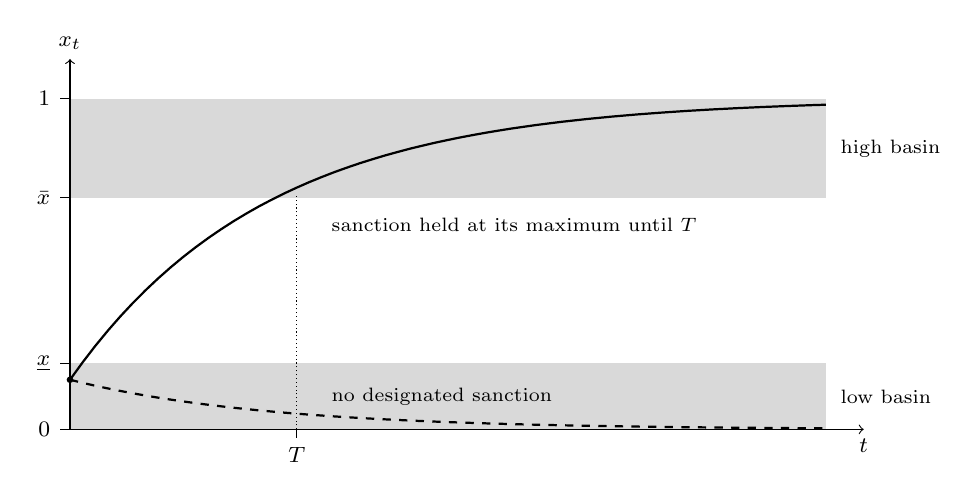
\begin{tikzpicture}[x=0.32cm,y=4.2cm,font=\footnotesize]
\fill[black!15] (0,0.7) rectangle (30,1);
\fill[black!15] (0,0) rectangle (30,0.2);
\draw[->] (0,0) -- (31.5,0) node[below] {$t$};
\draw[->] (0,0) -- (0,1.12) node[above] {$x_t$};
\foreach \y/\l in {0/0,0.2/\underline{x},0.7/\bar x,1/1} \draw (0,\y) -- (-0.4,\y) node[left] {$\l$};
\draw (9,0) -- (9,-0.025) node[below] {$T$};
\draw[densely dotted] (9,0) -- (9,0.71);
\draw[thick,domain=0:30,samples=61] plot (\x,{1-0.85*0.88^\x});
\draw[thick,dashed,domain=0:30,samples=61] plot (\x,{0.15*0.88^\x});
\fill (0,0.15) circle (1.2pt);
\node[anchor=west,font=\scriptsize] at (10,0.62) {sanction held at its maximum until $T$};
\node[anchor=west,font=\scriptsize] at (10,0.1) {no designated sanction};
\node[anchor=west,font=\scriptsize] at (30.2,0.85) {high basin};
\node[anchor=west,font=\scriptsize] at (30.2,0.1) {low basin};
\end{tikzpicture}
\caption{The path of the political state from the same start $x_0$ in the low basin
$[0,\underline x]$, under the partial-adjustment law. Dashed: without a designated
sanction the state stays in the low basin, where realized sanctions do not rise.
Solid: a sanction held at its maximum until date $T$ carries the state into the
high basin $[\bar x,1]$, after which equilibrium play keeps it there and the
sanction never falls (\Cref{prop:lock-in}).}
\label{fig:state-path}
\end{figure}

% @econ-contract paragraph
% id: DISC_BLUFFING
% role: Relate the designated sanction to bluffing under incomplete information (the author, 2026-10-17: "cite other paper's bluffing result ... they actually turn the bluffing to be true, and that caused the persist sanctions under this model"): a sanction imposed as a bluff, or to call one, and held long enough moves the state into the high basin, where continuing it is equilibrium play.
% depends_on: DISC_DESIGNATED_SANCTION
% handoff: Relief in practice.
% exact_ref: bib:Spaniel2015#pp=735-736,739
% source_role: bib:Spaniel2015#pp=735-736,739 => Under uncertainty about leader strength, weaker target leaders have incentives to bluff strength by continuing a crisis, and foreign powers sometimes call potential bluffs by implementing sanctions (read 2026-10-17 from the PDF); the bluffing result the paragraph builds on, not support for a result of this paper.
% exact_ref: bib:Brekhov2022#p=77
% source_role: bib:Brekhov2022#p=77 => Analyses targets' incentives to bluff under sanction (and reward) regimes in a repeated interaction with asymmetric information (read 2026-10-17 from the PDF); positioning only.
% exact_ref: tex-label:prop:lock-in
% support_status: VERIFIED
% status: PROPOSED
% @end-econ-contract
\central{Sanctions that begin as bluffs can become self-sustaining under equilibrium
play.} Under incomplete information, imposing sanctions can serve as a bluff or as a way
to call an opponent's bluff. In \citet[pp.~735--736]{Spaniel2015}, weaker target leaders
have ``incentives to bluff strength'' by continuing a crisis, and foreign powers respond
``by sometimes conceding and sometimes calling potential bluffs by implementing
sanctions''; \citet[p.~77]{Brekhov2022} analyzes target incentives to bluff under
sanctions. In those models, information revealed during the crisis determines subsequent
outcomes. Here, sanctions also shift the political state. A sanction imposed as a
bluff---or to call an opponent's bluff---and maintained for a sufficient duration acts as
a designated sanction in the sense defined above: it moves the state into the high basin,
where continued sanctioning is prescribed by equilibrium play. The bluff then becomes
self-fulfilling, and sanctions persist without any beliefs to revise.

\subsection{Real-world sanctions relief}
\label{sec:discussion:relief}
\label{sec:discussion:evidence}

% @econ-contract paragraph
% id: DISC_THREE_QUESTIONS
% role: Separate preference for relief, belief that it will be honoured, and its usability, and state the participation result (prop:relief-participation) at its scope, in words, as the model's answer to the first question.
% depends_on: DISC_BLUFFING
% handoff: Credibility of relief.
% merged_from: DISC_PARTICIPATION
% exact_ref: tex-label:prop:relief-participation
% support_status: NOT_APPLICABLE
% status: PROPOSED
% @end-econ-contract
\central{A natural application of the model is to proposals for sanctions relief, which raise
three related but distinct questions; the model's incentive comparisons speak to the
first.}\footnote{The participation
result is proved in \Cref{app:proofs:branch} of the Online Appendix; the economy
at which a temporary suspension of sanctions benefits a non-compliant target is recorded in the
formal supplement.}
Would policymakers prefer the arrangement and expect it to be honored, and would nominal
relief restore the economic activity it is intended to enable? On the first question,
consider a temporary suspension of sanctions followed by any equilibrium where the target
maintains full non-compliance, such as the constructed equilibrium. Under the
entrenchment condition and a sender response at full non-compliance that does not
decrease with the state, the change in incumbent payoffs does not support any date-zero
side payment between governments that would make the shock mutually acceptable. That
neither incumbent gains from such a shock follows jointly from three conditions: the
sender's positive marginal return to sanctioning a non-compliant target, the property
that compliance does not increase the sender's payoff at zero sanctions, and the
entrenchment condition. For an economy failing the entrenchment condition, a temporary
suspension of sanctions benefits a target that still does not comply.

% @econ-contract paragraph
% id: DISC_CREDIBILITY
% role: Tie the credibility of relief to commitment technologies and to lock-in, with the relief credibility point.
% depends_on: DISC_THREE_QUESTIONS
% handoff: Rival accounts of non-relief.
% exact_ref: bib:Powell2012#scope=paper
% source_role: bib:Powell2012#scope=paper => Already-cited source that singles out a costlessly reversible concession as least credible; it does not model this paper's state channel.
% support_status: UNVERIFIED
% status: PROPOSED
% @end-econ-contract
\central{The second question---whether relief will be honored---depends on commitment
technologies.} Lock-in depends on the initial state, and within a high basin resumed
equilibrium play generates no endogenous exit under the set and level conditions of
\Cref{prop:lock-in}. Expiry dates, review clauses, and other commitment technologies
operate by altering the strategic environment. Relief poses the hardest test for such
mechanisms. Relief that is reversible at no direct cost is the type that
\citet[p.~627]{Powell2012} identifies as least credible. In recent bargaining models of
war, the reliability of an agreement remains a parameter \citep{Ruggiero2026}. A full
model of relief institutions would need to specify, as separate primitives, who can
commit, who holds veto power, how private actors respond, and how these choices alter the
continuation game.

% @econ-contract paragraph
% id: DISC_RIVAL_ACCOUNTS
% role: Place rival accounts of non-relief without dismissing them as non-optimising (repair C6).
% depends_on: DISC_CREDIBILITY
% handoff: What the case material supports.
% exact_ref: bib:HalcoussisKaempferLowenberg2021#scope=paper
% source_role: bib:HalcoussisKaempferLowenberg2021#scope=paper => Already-cited legislative-cost account of sanction persistence; cited as an alternative, not as support for this model.
% support_status: UNVERIFIED
% status: PROPOSED
% @end-econ-contract
\central{Commitment problems are one explanation for persistent non-relief among
several; the model isolates a distinct mechanism.} In this mechanism, continued sanctions
can be optimal because of the state that sanctions have built, provided that the sender
values that target-side state and the entrenchment condition holds. Sanctions can be
optimal even if they are re-optimized every period and a lower sanction level is
feasible. Legislative constraints \citep{HalcoussisKaempferLowenberg2021}, administrative
persistence, and reputational incentives offer alternative explanations. Political or
reputational costs can themselves be incorporated into an optimizing decision
framework.

% @econ-contract paragraph
% id: DISC_PREDICTIONS
% role: State the two observable responses the classification separates, as model implications, not validation.
% depends_on: DISC_RIVAL_ACCOUNTS
% handoff: The case material.
% exact_ref: tex-label:thm:four-cells
% support_status: VERIFIED
% status: PROPOSED
% @end-econ-contract
\central{Comparisons across constructed equilibria distinguish two observable responses
to a single sanctions regime: greater compliance and deeper entrenchment.}\footnote{The
model's predictions are collected in \Cref{app:moved-ah} of the Online Appendix,
and the case sources' discussion of evasion and enforcement in
\Cref{app:moved-ad}.} Greater
compliance arises when the target's forward-looking incentive is weak and a
forward-looking sender raises the cost of relief; deeper entrenchment arises when that
incentive is strong and a forward-looking sender raises the steady-state level.

% @econ-contract paragraph
% id: DISC_CASE_MATERIAL
% role: Use the already-cited case material as motivation for the mechanism, with the Sender's stake kept as a maintained restriction.
% depends_on: DISC_PREDICTIONS
% handoff: The relief cases.
% exact_ref: bib:HaggardNoland2017#scope=paper
% source_role: bib:HaggardNoland2017#scope=paper => Already-cited account of an authoritarian target passing sanction costs to citizens; motivates the mechanism, does not identify any parameter.
% exact_ref: bib:UNPanelDPRK2024#scope=paper
% source_role: bib:UNPanelDPRK2024#scope=paper => Already-cited report of tighter control under sanctions; motivation only.
% support_status: UNVERIFIED
% status: PROPOSED
% @end-econ-contract
\central{North Korea, a context in which this feedback mechanism may be salient, helps
motivate the analysis.} \citet{HaggardNoland2017} describe an authoritarian target able
to pass sanction costs onto its citizens and a leadership reluctant to weaken its control
over foreign economic activity; in the model's terms, these correspond to low sanction
pain and a high valuation of the state---the two sides of the entrenchment condition. A
United Nations Panel of Experts report documents tighter economic, social, and political
controls and more centralized economic management under sanctions
\citep{UNPanelDPRK2024}. These same sources document evasion, enforcement, and
coordination challenges, which can coexist with the political-state feedback
mechanism.

% @econ-contract paragraph
% id: DISC_CASE_RELIEF
% role: Use the Iranian and Russian relief material (note N134, promoted 2026-10-02) to separate acceptability, credibility and delivery of relief, as motivation only.
% depends_on: DISC_CASE_MATERIAL
% handoff: The limits of the equilibrium interpretation.
% exact_ref: tex-label:sec:discussion:relief
% exact_ref: bib:BajoghliNasrSalehiIsfahaniVaez2024#pp=115-116,121-123
% source_role: bib:BajoghliNasrSalehiIsfahaniVaez2024#pp=115-116,121-123 => The authors' account (read 2026-10-02) that the prospect of lifting brought Iran to the 2015 agreement while rollback was slow, could be blocked or reimposed through Congress, and was made immaterial by remaining financial sanctions; motivation for separating the three relief questions, not a test of the model.
% exact_ref: bib:SnegovayaFentonDolbaiaBergmann2025#pp=26,31-32
% source_role: bib:SnegovayaFentonDolbaiaBergmann2025#pp=26,31-32 => The report's description (read 2026-10-02) of Russian businesses that thrive under isolation and fear returning competition, against firms that would gain from partial relief, with its scenario assumptions; heterogeneous interests, projections rather than observed outcomes.
% support_status: UNVERIFIED
% status: PROPOSED
% @end-econ-contract
\central{Iran and Russia illustrate all three questions raised above.} According to
\citet[pp.~115--116]{BajoghliNasrSalehiIsfahaniVaez2024}, the prospect of earlier
sanctions being lifted---not the threat of additional sanctions---brought Iran to the 2015
agreement. Yet the rollback was gradual and required political support at multiple levels
of the United States government. Congress, which is often involved in delisting
decisions, could impose additional hurdles or reimpose the same sanctions under another
pretext, and sanctions remaining on Iran's financial and banking system made the lifting
of others immaterial (pp.~121--123). Accepting relief, expecting it to be honored, and
being able to benefit from it are therefore distinct margins. In Russia, businesses that
have thrived under reduced competition fear the return of Western competitors, while
import- and export-dependent firms could gain from partial sanctions relief
\citep[pp.~31--32]{SnegovayaFentonDolbaiaBergmann2025}. The report's scenarios are
projections from 2025 (p.~26). This heterogeneity is what the political state variable
summarizes.

\subsection{Scope and limitations}
\label{sec:discussion:scope}

% @econ-contract paragraph
% id: DISC_SCOPE
% role: State the mechanism the model isolates and the object of its theorems for a specified instrument and compliance demand; effectiveness judged against a sender's objectives; how the class specializes to other coercive systems.
% depends_on: DISC_CASE_RELIEF
% handoff: The equilibrium concept and the results that reach beyond the constructed equilibria (repair C2).
% exact_ref: bib:GAO2025RussiaSanctions#pp=14
% source_role: bib:GAO2025RussiaSanctions#pp=14 => The report's three categories of objectives (read 2026-10-02); names the objectives against which effectiveness is judged, supports no model result.
% support_status: NOT_APPLICABLE
% status: PROPOSED
% @end-econ-contract
\central{We have deliberately isolated one public-choice mechanism behind persistent sanctions:
sanctions strengthen the target-side constituency that supports their continuation, and
both governments value that constituency.} Within the class, compliance affects the
sender by reducing its incentive to sanction. Given a coercive instrument and a
compliance demand, the theorems characterize how equilibrium play evolves from the
political state that sanctions---once imposed---have altered. Effectiveness, by contrast,
is measured against a sender's objectives, which the U.S. Government Accountability
Office identifies for U.S. measures on Russia as economic pressure, inhibition of the war
effort, and accountability \citep[p.~14]{GAO2025RussiaSanctions}. The mathematical
structure of the class can be adapted to other coercive systems. Doing so requires
mapping their actions, constituency effects, and payoff signs into the class structure,
including analogues of each government's stake in the state and of the entrenchment
condition.

% @econ-contract paragraph
% id: MODEL_EQUILIBRIUM_SCOPE
% role: How existence is obtained (by construction on invariant sets of value functions), and the concept against strong stationary Stackelberg and history-dependent equilibria (moved from Section 2.4, 2026-10-16, structure plan S4).
% depends_on: DISC_SCOPE
% handoff: The objects solved jointly and the results beyond the constructed equilibria.
% exact_ref: tex-label:thm:existence
% exact_ref: bib:HeLiuChen2025#scope=paper
% source_role: bib:HeLiuChen2025#scope=paper => Already-cited dynamic feedback Stackelberg existence and computation antecedent (restored 2026-10-02 after the rebuild dropped it); positions the joint-iteration existence route, does not prove it.
% exact_ref: bib:LiSojoudiTomlinFridovichKeil2024#scope=paper
% source_role: bib:LiSojoudiTomlinFridovichKeil2024#scope=paper => Already-cited feedback Stackelberg computation antecedent (restored 2026-10-02 after the rebuild dropped it); positioning only.
% exact_ref: tex-label:prop:history-deviations
% support_status: VERIFIED
% status: PROPOSED
% @end-econ-contract
\central{Existence is established by construction, and each construction pins down its
equilibrium only within the sets of value functions it employs.} Where the results
construct a value function, it is the unique fixed point of its Bellman operator defined
over an explicitly stated \emph{invariant set of value functions}: a closed set with
stated bounds on the level and slope of each member (and on
curvature for the sender), which the operator maps into itself. \Cref{sec:results} constructs
equilibria over the full class of economies. A general existence argument---based on
joint contraction of both Bellman equations when the coupling between them is
sufficiently weak---follows in the spirit of \citet{StokeyLucas1989} and of broader
research on the existence and computation of dynamic feedback Stackelberg equilibria
\citep{HeLiuChen2025,LiSojoudiTomlinFridovichKeil2024}.

\central{Two comparisons delineate the scope of the equilibrium concept: with the
stationary strong Stackelberg equilibrium, and with history-dependent strategies.}
First, target optimality in $\mathcal E$ is pointwise: at each state, the target
maximizes the right-hand side of \eqref{eq:T-bellman}, taking continuation values as
given. In a stationary strong Stackelberg equilibrium, by contrast, the leader selects an
entire policy function and anticipates that the follower re-optimizes after every policy
deviation; the two concepts need not coincide \citep{Bucarey2023,KudoAkimoto2026}. The
equilibrium concept is time-consistent because both governments re-optimize at every
state. Second, against any equilibrium in $\mathcal E$, no pure strategy conditioned on
the entire history outperforms the equilibrium's own play, from any initial state
and---for the sender---after any observed compliance level on or off the equilibrium
path.

% @econ-contract paragraph
% id: DISC_EQUILIBRIUM_LIMITS
% role: State the equilibrium notion, the objects it solves jointly, and the two results that reach beyond the constructed equilibria (repair C2).
% depends_on: MODEL_EQUILIBRIUM_SCOPE
% handoff: Levels of generality.
% merged_from: DISC_ENDOGENOUS
% exact_ref: tex-label:prop:security
% note: 2026-10-16 (structure plan S4): the Markov sentence is in Section 2.4 and the minmax and uniqueness results in Section 3.4; this paragraph points there.
% support_status: VERIFIED
% status: PROPOSED
% @end-econ-contract
\central{Within each equilibrium, the target's compliance rule, the sender's sanction
rule, both value functions, both feedback policies, and the political-state trajectory
are solved jointly.} In the interest-group polity, the pressure levels of competing
groups also constitute a Nash equilibrium of the political contest. Two results extend
beyond the constructed equilibria under the strong entrenchment condition: the target's
minmax payoff bound and the uniqueness of full non-compliance among non-decreasing
sanction rules (\Cref{sec:results:security}).

% @econ-contract paragraph
% id: DISC_GENERALITY_LEVELS
% role: Separate results about every equilibrium satisfying stated conditions, results derived from primitives on the class, and results established at example economies, citing main-text results only.
% depends_on: DISC_EQUILIBRIUM_LIMITS
% handoff: Open extensions.
% exact_ref: tex-label:prop:certified-equilibria
% support_status: VERIFIED
% status: PROPOSED
% @end-econ-contract
\central{The results operate at three levels of generality.} First, some apply to every
equilibrium satisfying stated conditions: lock-in (\Cref{prop:lock-in}) applies to every
equilibrium meeting its basin conditions and, for entry, its transition conditions; the
fixed-target-policy comparison (\Cref{thm:dominance}) applies to every non-decreasing
sender value at every state, and thus to every equilibrium containing one; the premium bound
of \Cref{sec:results:wedge} applies to every equilibrium with a non-increasing target
policy, for economies in the class with an upper bound on the substitution rate at which
larger concessions are never worth more to the sender at zero sanctions; and the minmax
bound applies to every equilibrium in $\mathcal E$. Second, the myopic-benchmark
comparison (\Cref{thm:regime-separation}), the four-case characterization
(\Cref{thm:four-cells}), and the threshold result (\Cref{prop:collapse-threshold}) derive
equilibrium properties and dynamics from inequalities across primitives over the class, and
greater target patience preserves the full-non-compliance equilibrium that exists at a
lower discount factor (\Cref{prop:patience-existence}). The welfare results of
\Cref{sec:welfare} hold across the class, as do the rescaling property and the planner
optimality condition for any representation and any bounded welfare flow. Third, some
results are established via example economies, which demonstrate that hypotheses can be
satisfied or bounds attained: the welfare loss in one interest-group polity
(\Cref{sec:welfare:efficiency}), the attainment of the premium bound
(\Cref{sec:results:wedge}), and economies satisfying the lock-in conditions
(\Cref{app:persistence:reading} of the Online Appendix).

% @econ-contract paragraph
% id: DISC_OPEN
% role: Name the extensions and the measurement requirements for empirical work.
% depends_on: DISC_GENERALITY_LEVELS
% handoff: The conclusion.
% exact_ref: bib:AttiaGrauvogel2023#scope=paper
% source_role: bib:AttiaGrauvogel2023#scope=paper => Already-cited exploratory association between institutional clauses and termination; not a causal estimate and not support for a model result.
% support_status: UNVERIFIED
% status: PROPOSED
% @end-econ-contract
\central{Two broad kinds of extensions build on these results: empirical measurement of
the political state and its associated payoff terms, and richer theoretical models of
the state and of relief institutions.} Disciplining estimates of the political-state
transition and the payoff terms governing basin entry would require empirical measures
that separate the political state from aggregate income, and distinguish within-target
adjustment from selection across surviving episodes. Theoretical extensions could
incorporate multidimensional political states, stochastic shock duration,
forward-looking investment by groups in their own future power
\citep{AcemogluRobinson2008}, or explicit relief and commitment technologies. The last of
these could alter entry into or create exit from the high basin, and
\citet{AttiaGrauvogel2023} document exploratory empirical associations between such
provisions and sanction termination. A fully optimal relief policy would require explicit
institutional instruments and commitment constraints. A symmetric framework in which both
governments directly move the state---of the kind \citet{Powell2013} calls for---would
embed compliance directly into the transition law and require rederiving the argument
that compliance reduces the sender's incentive to sanction.
